\documentclass{article}
\usepackage{graphicx}
\usepackage{times}
\begin{document}

\title{Open Diameter Software Architecture}
\author{Victor Fajardo and Yoshihiro Ohba}
\date{August 26, 2002}
\maketitle

This white paper describes the software architecture taken by Open
Diameter in implementing the Diameter base protocol\cite{basep}.  This
architecutre is geared towards achieving a modular, extensible and
thread-safe solution for Diameter implementation.

\tableofcontents
\pagenumbering{arabic}
\pagebreak

\section{Overview\label{sec:overview}}

The architecture of the Open Diameter implementation borrows heavily
from the design patterns developed in ACE \cite{ace}. In particular, the
socket acceptor, connector and thread pooling patterns are employed. In
addition to using ACE based patterns, the OS abstraction layer provided
by the ACE library is heavily utilized in this implementation. This
document will concentrate on the overall architecture of the Open
Diameter libraries and detailed implementation is not described in this
document.  Especially, the focus will be on the ACE patterns used in the
Open Diameter implementation.

\subsection{Programming Language\label{sec:language}}

The programming language of choice is C++. It is our intent to take
advantage of object methodology, widespread familiarity and abundant
support offered by C++. In addition, a decision was made to utilize
standard C++ libraries to allow for speed of development.  C++ also
becomes a necessity to support highly preferred development tools such
as ACE which is implemented only in C++.

\subsection{Platform/System Support\label{sec:platform}}

Care has been given to allow the code to be as platform independent as
possible. All system calls are abstracted by an utilities provided by
ACE. In addition all system calls not covered within the base ACE OS
abstraction layer are made as POSIX compliant as possible. With the
integral use of ACE, supported platforms for the Open Diameter library
will fall within the supported platforms of ACE.

%\section{Diameter Implementation\label{sec:implementation}}

\section{Modules and Libraries\label{sec:modules}}

The current architecture of Open Diameter software is divided into four
(4) logical modules. An application core, a session management module, a
transport management module and a message parsing module. These first
(3) modules comprise a Diameter base protocol engine and is contained
within a single library (libdiameter). The message parsing module is
implemented as a separate library (libdiamparser) so that it can be used
for application programs that utilize AAA services to communicate with
the Open Diameter program by using the Diameter message format.
These two libraries are written in C++ and provide the Diameter C++ API
\cite{api} to provide applications the functionalities of the Diameter
base protocol \cite{basep}.

Figure~\ref{fig:modules} shows the relationship between the logical
modules and applications.


\begin{figure}[htbp]
\center{
\leavevmode
\includegraphics[scale=0.8]{figs/modules.eps}
\caption{Diameter Library Modules\label{fig:modules}}
}
\end{figure}

As shown in Figure~\ref{fig:modules}, the Diameter message parser
library (libdiamparser) is implemented as a separate library from the
library for the Diameter base protocol engine (libdiameter).  Both
libraries are common to any client or server authentication application
that uses them. Details of all logical modules are described in the
succeeding sections.

\subsection{Application Core\label{sec:appcore}}

The application core is a central storage for all global data and for
initialization and termination services for the entire Diameter
library. For each application wishing to use the library, an instance of
the application core has to be created. This is reflected in the design
of the draft API \cite{api}. As shown in Figure~\ref{fig:modules}, whether
the user application is a client or server authentication application or
a mere proxy/relay application, an instance of the application core is
required. Since an application core is heap based memory, it is possible
in certain cases to create multiple instances of an application cores
within a single program. However, it is recommended that a single
application core be created for each software program since there will
be a likely contentions over the transport level listening ports with
which each application core needs to listen to.

Included in the global data store of the application core are all the
static data contained in the XML configuration files
(Section~\ref{sec:configuration}). The session database, peer services
which houses the peer and routing tables, application subscription list
and the factory are all referenced here.  The initialization of the
application core is achieved via its encompassing class
(AAAApplicationCore) as specified in the draft API
\cite{api}. Initialization involves startup of the factory (master
thread, Section~\ref{sec:mastert}), loading of configuration files,
etc. Termination of the application core would be the symmetric opposite
of the operations in initialization. However, some wait states are
needed in termination to ensure that all existing threads exits
properly.

\subsection{Transport Manager\label{sec:transport}}

The transport manager is an integral partner of the application
core. Its main responsibility is to maintain connection states with
other Diameter peers (which includes recovery) as well as routing and
delivery of Diameter messages. Delivery of local Diameter messages,
i.e. those for local sessions, means that the transport management
module passes the message to the session manager.

With the introduction of ACE communications acceptor/connector pattern,
the implementation of the transport manager revolves around ACE service
handler classes (Section~\ref{sec:peert}). As noted in
Section~\ref{sec:peert}, the factory resides in the application core and
hence the ACE acceptor and connector object are actually serviced within
the factory (master thread, Section~\ref{sec:mastert}). A singleton
class acts as initializer and terminator for the transport management
module (Section~\ref{sec:peert}). Since connection activity details
reside within ACE, the service handlers can concentrate on the main
functions that the transport manager is responsible for.

As shown in Figure~\ref{fig:modules}, in using the Diameter library, the
transport management module will always be required by the application
core no matter what type of application uses the library. Since there is
no need for the application to interact with this module the draft API
\cite{api} has no direct reference to this module. It is a hidden yet
integral module which all upper level modules require.

\subsection{Session Manager\label{sec:session}}

The session management module is responsible for storing and maintaining
Diameter sessions for client/server authentication application using the
Diameter library. A red-black tree serves as a database of sessions
keyed by session id's \cite{basep}. Each session stores the current
session state, active timers and other session related
information. Since an application relates to the Diameter library via
sessions, the draft API \cite{api} exposes necessary functionality in
manipulating a session. It also relates transmission of messages from
the an application via an existing session hence associate every
application generated message will be associated with a session.

As noted in Section~\ref{sec:pool}, the execution context of the
session manager is based upon a thread pool. So each session in the
database also contains a job queue that enables the thread pool to
serially execute all the necessary events for a given session. The
session database itself as well as the job queues
(Section~\ref{sec:session}) for each session is protected by mutex
locks. As noted in Section~\ref{sec:appcore}, the session database is
part of the application core but the underlying methods and functions to
maintain the state of each session are in the session management
module. Interaction between session manager and transport manager is
discussed in detail in Section~\ref{sec:msgtransport}.

\subsection{Message Parser\label{sec:msgparser}}

The message parser module is used for parsing Diameter messages
including header and payload, where the payload part is consist 
of Diameter AVP(s).

In the message parser module, all known AVP's and command codes are
loaded into memory during initialization phase via the dictionary files
to construct a runtime dictionary database.  These dictionary files,
like configuration files, are XML based. The XML format is well known
and hence very well supported.  Apache's Xerces C++ XML library is used
to parse the dictionary files. It is open source library which is
heavily utilized in the apache web environment.  Extendibility of the
dictionary will be provided with the use of XML.

Mutual exclusion protection is not necessary for the runtime dictionary
database despite serving a threaded environment since all access to it's
runtime database is read-only.


\section{Threaded View of the Architecture
\label{sec:architecture}}

The threaded view of the entire architecture for the Open Diameter
implementation is shown in Figure~\ref{fig:architecture}.

\begin{figure}[htbp]
\center{
\leavevmode
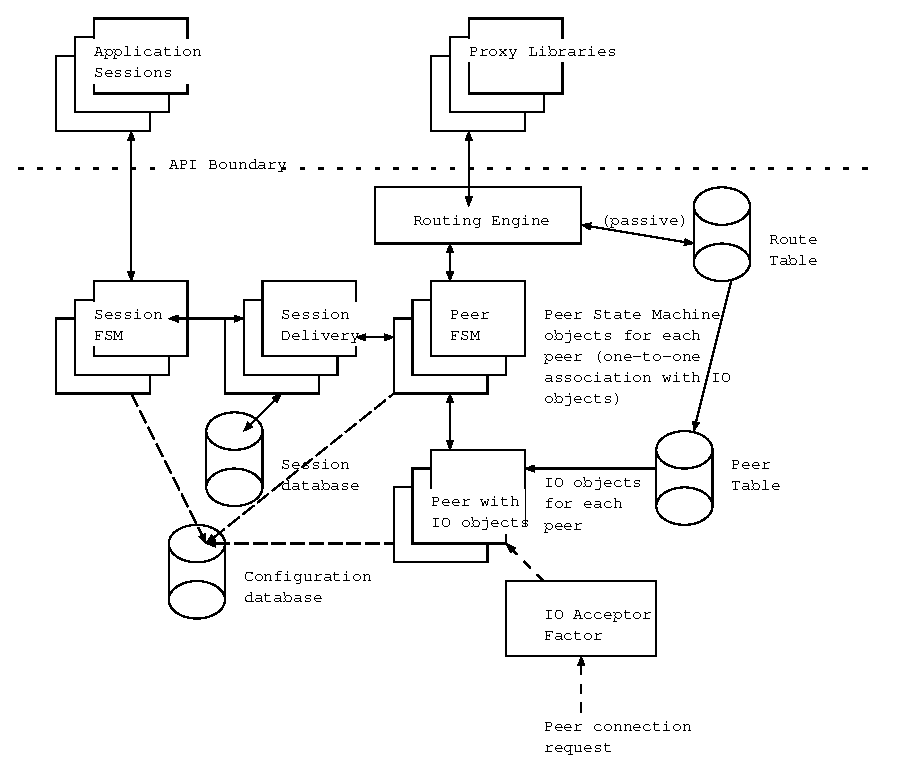
\includegraphics[scale=0.8]{figs/architecture.eps}
\caption{Threaded View of Open Diameter Architecture\label{fig:architecture}}
}
\end{figure}

As shown in the Figure~\ref{fig:architecture}, the execution context for
Diameter protocol functions are provided by multiple threads. The thread
handling are based on the ACE thread implementations. The issue of
contention and serialization between components within the
implementation is solved by using protected queues. As with threading,
the queue and locks (which provided protection) are ACE based. Note that
the ACE classes used in the libdiameter library will be mentioned in
this document. However, it is assumed that the reader is familiar with
these ACE classes. Detailed description of these classes is best served
by ACE\cite{ace}.

As shown in Figure~\ref{fig:architecture}, several threads exist within
the Diameter program.  Each of these threads are based on ACE
thread/task classes which not only provides platform abstracted
threading but also a software design pattern that strictly defines the
boundaries of an executing module. Within each thread, a protected
message queue exist that allows threads to pass pre-formed messages to
each other. For the purpose of the Diameter implementation, these queues
will be termed job queues. Further discussion on the use of job queues
are described in the types of threads that exist in the program. These
are as follows:

\subsection{Master Thread\label{sec:mastert}}

A master thread exists to orchestrate the existence of all other threads
in the program. The master thread, also known as the factory, is
responsible for spawning a thread for each active peer connection (both
for connected or accepted communication request) It has the
responsibility of initiating and monitoring local asynchronous
connection request as well as accepting remote connection request. On
success of any of these request, it spawns a thread for the newly
established connection and passes ownership of the connection to the new
thread. An advantage of using ACE for this specific communications
pattern is that the underlying communication transport used is
independent of this pattern. Meaning that the thread spawning behavior
based on successful connections will remain the same whether using TCP
or SCTP as an underlying transport.

The factory is also responsible for maintaining the existence of a
thread pool. This thread pool is used as a load balanced execution
context for session management. Beyond being created and destroyed the
factory, the threads in the pool is fairly independent of the
factory. Details about the thread pool and its role is discussed in the
succeeding topics Section~\ref{sec:architecture}. In addition, the
factory also provides global timer services for all internal timing
needs.  All timer requests are callback based and this global timer runs
within the context of the master thread.

\subsection{Peer Connection Threads\label{sec:peert}}

As mentioned in Section~\ref{sec:mastert}, the factory spawns a thread
to handle each successful peer connection. The responsibility of a peer
thread is to adhere to the peer state machine as stated in the Diameter
draft \cite{basep}, to send and receive Diameter messages destined for
other peers (forwarding) or local processing (session management), to
maintaining the peer table and other functions necessary for
establishing Diameter peer connection.

In libdiameter, a singleton class (AAAPeerService) exist to service the
initialization and termination requirements for transport management. In
this singleton class, the peer table is examined to see if a connections
to locally configure peers be attempted on startup. If so requests are
made to the master thread to initiate asynchronous connection to the
peers. These pending connections are monitored by the master thread for
success or failure. On success, a peer thread is spawned and ownership
of the newly established connection is passed to the thread. In
addition, the singleton contains globally accessible protected databases
that each peer thread requires, i.e. the routing table and the peer
table.

For incoming connections, the master thread is constantly monitoring the
well known Diameter port for connection request. Once, a connection
request is received, a peer thread is spawned. As with connection
attempts, the ownership of the established connection is passed
on. Regardless of whether, connecting or accepting, the peer threads
design pattern is the same. An established connection needs to be
serviced within the thread. The Diameter peer state machine, which is
independent of the design pattern, will dictate the behavior of the
executing thread based on whether it connected or accepted the
request. As an example, in the case of accepted request, the state
machine would need to wait for a complete CER to arrive then determine
whether to accept the peer or not. If accepted, the peer thread may add
this new peer as a dynamic entry into the peer table. As for connecting
peers, it would need to send the CER on start of the state machine.

Since ownership of the connection is passed on to the peer thread, it is
it's responsibility to formally disconnect or handle disconnection
events from the remote peer. These events are common and thus part of
the design pattern. The ACE design pattern used are based on
\begin{verbatim}ACE_Svc_handler\end{verbatim} template class. Also,
since each peer thread has a message queue built in, it has to
constantly monitor the message queue and the established peer connection
and act accordingly once a message from any of those sources appear.

\subsection{Thread Pool\label{sec:pool}}

The thread pool design pattern exists to facilitate the use of load
balancing in session management. All required Diameter protocol
activities beyond the peer task will be performed by a thread in this
pool. The pool is composed of a collection of threads that constantly
monitors a job request queue as shown in
Figure~\ref{fig:architecture}. The job request queue is protected by a
mutex lock that allows only one thread to dequeue an entry at a
time. The entries in these queue contains specific job instructions as
well as data, i.e. parsing a message, look up a session and switch its
state machine, call user subscription etc. The ability to send
instructions, along with any associated data, via this queue gives the
opportunity to assign a pending job to the next available idle
thread. Parallelized load balancing on a fair, first come first serve
basis based on the mutex lock can then be achieved.

The contents of the job queues are generic enough to allow instances of
objects to be enqueued and dequeued. With this ability, a design pattern
based on job instance is used to as a generic way of sending
instructions and data to a thread in the pool for processing. In the
implementation, a job instance is defined as follows:

\begin{figure}[htbp]
\begin{center}
\begin{verbatim}
class AAAJobInstance {
   public:
      AAAJobInstance(void *p) { payload = p; };
      virtual u_int32_t Job() { return (0); };

   protected:
      void* payload;
};
\end{verbatim}
\caption{Generic job instance base class {\bf AAAJobInstance}\label{fig:jobsource}}
\end{center}
\end{figure}

The AAAJobInstance class is used as a base class for purpose specific
derived classes, i.e., message parsing class, timeout event processing
class, etc. As an example, a message parsing class can override
AAAJobInstance and implement the Job() method where actually parsing is
to be done. The raw message itself is reference by payload.  This
derived class can then be injected into a job request queue and the next
idle thread in the pool can dequeue the job instance and invoke it's
Job() method. Hence, all threads in the pool monitors the job request
queue and waits to dequeue the next available job instance so they can
invoke it's Job() method. To continue the parsing example, once the
message has been parsed, the Job() method may also try to determine if
the belongs to an existing session. If it does, it creates a session
message job instance and enqueues it to the job request queue so that
the next available thread can process switch the session state machine
based on the parse message.

The granularity of the task that each Job() method must perform is
restricted to a very specific function. The success of a load balanced
system depends on how well distributed and finely divided each job
is. In libdiameter, the number of threads in the pool is controlled by
local configuration.

\section{Basic Message Processing\label{sec:processing}}

This section describes how incoming and outgoing messages are processed
by the transport and session manager and the message parser so as to
provide more insight to the Open Diameter software architecture.

\subsection{Message Transport and Session Processing\label{sec:msgtransport}}

An incoming message from a remote peer is initially received and
processed by the transport manager within one of the peer threads
servicing the remote peer. Once fully received, the transport manager
can partially parse the header and parts of the message body if needed
to determine where to forward the message. If the message is for another
remote host, the message is enqueued into the job queue of the peer
thread servicing the destination peer. If the message is for local
consumption, the transport manager passes the message to the session
manager by injecting the message into the message parsing job queue, see
Figure~\ref{fig:architecture}. This queue serves as the logical boundary
between the transport manager and session manager on the ingress
path. Once a message is enqueued into the message parsing job queue, a
new thread pool job request is made so that entries in the message
parsing job queue can actually be processed. This new job request is
injected into the thread pools job request queue where the next
available thread can dequeue it and start processesing. On processing,
the message is dequeued from the message parsing job queue and then
completely parsed and passed on directly to the application subscriber
who has specifically registered to receive such a message. After
invoking the application subscription, the job is completed.

Within the subscription, an application may need to query the session
database using the message.  The query will return the appropriate
session object associated with the message. The session object can then
be used to update the session state machine or transmitt a reply to the
received message.  If the parsed message, however, is a base protocol
message used for use only by the Diameter library (ASR,ASA,STR,STA),
then the message subscription is internal, i.e. the library itself
subscribes for those base protocol messages. And hence, the subscription
invocation is also internal and any adjustments that this subscription
makes to the session state machine follows the same process of creating
a new thread pool job request and injecting it into the thread pool job
request queue. This new job is a session job which is again waiting to
be processed by the next available thread in the pool. Once dequeued by
an available thread then updates to the session state machine based on
the associated message can be made.

For outgoing messages generated by an application, the application
invokes a Diameter API transmission class which associates the message
to a session. This involves enqueuing the message to the job queue of
that session. Again, a new thread pool job request is created and
injected into the thread pool job request queue. Once dequeued by the
next available thread, the job performs all necessary update to the
session state machine based on the outgoing message if necessary and
then enqueues the message to the job queue of the peer thread where this
message is destined for. The job queues for the peer threads, also known
as transmit queue as shown in Figure~\ref{fig:architecture} is the
logical boundary between the session manager and the transport manager
on the egress path. This same job determines which transmit queue the
message is to be injected to by querying the transport manager peer
table. Once enqueued into the transmitt queue of the peer thread, the
peer thread can compose the message into a raw buffer and transmit it
via it's established connection.

Internally, each peer thread has an internal pending message queue in
addition to it's transmitt queue. The pending message queue shown in
Figure~\ref{fig:architecture}, is where all transmitted but
un-acknowledge messages are stored, i.e. transmitted request messages
that is still awaiting a correspoding answer message. As specified in
Section 5.5.4 of the Diameter draft \cite{basep}, this is used in
failover procedure. Since each peer connection resides within it's own
thread context, detection of transport failure with the remote peer and
immediate failover is done internally within the thread. Failover is
easily accomplised simply by flaging and transferring all the messages
in the pending message queue into the transmitt queue of the peer thread
of an alternative server. However, the architecture dictates that once a
transport connection for a peer thread closes or fails, the peer thread
has to exit. This means that in order to perform failback, the peer
thread schedules a connection retry with the factory request before the
peer thread exits. The scheduling is done via timer request. Once the
timer event occurs, a connection attempt is made by the factory. Once a
connection is re-established with the peer, a new peer thread is started
by the factory and communication with the remote peer is once again
possible. If the re-connection attempt fails, another connection retry
is scheduled and the process is repeated.

\subsection{Message Parsing\label{sec:msgparsing}}

Diameter message parsing can occur at least in the following cases.

\begin{itemize}
 \item When a Diameter message is received from a peer, the transport
 manager needs to parse the message in order to determine whether the
 message should be queued in the message parsing queue for further
 processing by the session manager or forwarded to another Diameter
 node.  In this case, only specific AVPs such as Destination-Host AVP
 and Destination-Realm AVP need to be parsed instead of fully parsing
 against the command dictionary.
 \item When a received Diameter message is processed by the session
 manager, the message is fully parsed against the dictionary by the
 session manager and passed to an appropriate application message
 subscription handler for application specific processing.
 \item When a Diameter message is generated by the application via an
 application subscription handler or by the transport manager, the
 message needs to be constructed by using the message parser module.  In
 this case, the message is fully parsed against the dictionary and
 passed to the transport module.
 \item When a Diameter message generated by the application is sent to a
 peer, the message needs to be parsed by the transport manager in order
 to determine the peer to send the message.  In this case, only specific
 AVPs such as Destination-Host AVP and Destination-Realm AVP need to
 be parsed.
\end{itemize}

For all of above cases, the same date structures are used regardless of
whether parsing is performed for message assemble or disassemble.  The
data structures used for message parsing are container list ({\tt
AAAAvpContainerList}), container\\ ({\tt AAAAvpContainer}) and container
entry ({\tt AAAAvpContainerEntry}).  An example pointer chains of those
data structures are shown in Figure~\ref{fig:parser}.

When assembling or disassembling a message, a container is assigned for
each type of AVP and attached to a container list.  Also, a distinct
container entry is assigned for each AVP that is included (when
disassembling) or to be included (when assembling) in the message and
attached to the container of the corresponding AVP type.  The parent
container list needs to be provided by the application.  When
disassembling a message, either the application or the parser module has
the responsibility of assignment and attachment of containers, but only
the parser module has the responsibility of assignment and attachment of
container entries.  On the other hand, when assembling a message,
applications have the responsibility of assignment and attachment of
containers and container entries.  In any cases, application is the only
entity that have the responsibility of releasing and detaching
containers and container entries.

Assignment and release of containers and container entries is done via
container manager ({\tt AAAAvpContainerManager}) and container entry
manager\\ ({\tt AAAAvpContainerEntryManager}), respectively.  Resource
management for containers and container entries is based on
pre-allocation (instead of on-demand allocation via malloc() system
call) in order to avoid frequent memory allocation/deallocation.

AVP data in a Grouped AVP is stored in a distinct container list for
which a pointer is stored in the container entry for the Grouped AVP.
In other words, a Diameter message payload and a Grouped AVP is treated
in the same manner.  It is also possible to process nested Grouped AVPs
in which a Grouped AVP contains another Grouped AVP as its element AVP.

The Open Diameter thread architecture is designed such that a message is
always exclusively processed by a single thread.  Resource access
contention among multiple threads for message parsing is only possible
when assigning and releasing containers and container entries.  To
eliminate the contention, mutex protection is provided inside the
container and container entry managers.  Thus, applications are not
required to provide their own mutex protection mechanism for message
parsing.

\begin{figure}[htbp]
\center{
\leavevmode
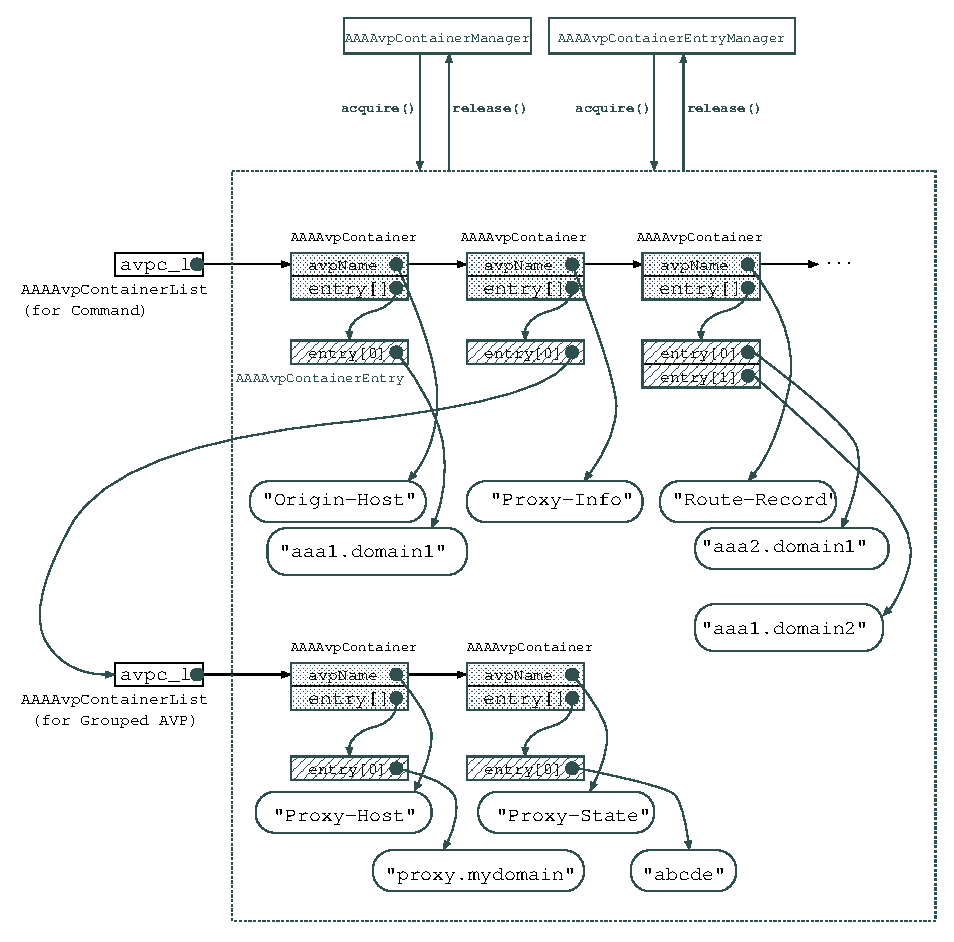
\includegraphics[scale=0.8]{figs/parser_structure.eps}
\caption{Diameter Message Payload Parsing Structure\label{fig:parser}}
}
\end{figure}

Open Diameter defines a template parser class named {\tt AAAParser}
which provides a unified way to parse any data structure.  Any {\tt
AAAParser} class object consists of the following members.

\begin{description}
 \item[Raw data] less-structured data such as string buffers.
 \item[Application data] structured representation of raw data, such as
	    AVP container list.
 \item[Dictionary data] Data that describes a rule for data conversion
 between raw data and application data.  Dictionary data can be null.
 \item[Data set/get functions] A set of functions used for
 setting/getting raw data, application data and dictionary data to/from
 the parser.
 \item[Message parsing and data conversion functions] A pair of
 functions used for data parsing and conversion between raw data and
 application data.
\end{description}

In fact, a number of parser classes are defined for parsing different
objects including Diameter header, Diameter payload, AVP header and AVP
payload of each data type, by specializing the template {\tt AAAParser}
class.

\subsubsection{Registering New AVP Types\label{sec:avpparsing}}

Open Diameter parser library defines an API to define a new AVP type and
a parser to parse the new type, in addition to the default supported AVP
types such as Integer32, Unsigned32, OctetString, UTF8String, Grouped
and IPAddress.  This feature is particularly important not only for
developing new Diameter applications and but also for developing a new
protocol that uses Diameter AVP formats.  PANA (Protocol for carrying
Authentication for Network Access) is an example of the latter case.

Registration of a new AVP type can be done via adding a new AVP type
entry called {\tt AvpType}, where an AVP type entry consists of the
following members.

\begin{description}
 \item[Type name] the name of this AVP type.
 \item[Type code] an integer that is used by the parser library for
 distinguishing this AVP type.  The type code must be unique among all
 the types in the system.  The type code is used only inside the library
 and never carried in Diameter messages.
 \item[Type size] the minimum size of the data of this AVP type.  This
 information is used for creating an placeholder AVP when a certain
 class of error occurs.
 \item[Dictionary data] data that describes a rule for data conversion
 between raw data and application data.  Dictionary data can be null.
 \item[Parser creator] a function object or a functor that is used for
 creating a parser class instance that parses the data of the AVP type.
 \item[Container entry creator] a function object or a functor that is
 used for creating a container entry that contains the data of the AVP
 type.
\end{description}

The list of {\tt AVPType} instances are retained in an AVP type list
{\tt AAAAvpTypeList}, which is a singleton.


\subsection{Configuration\label{sec:configuration}}

All configuration files for the Open Diameter library, as with the
parser library, are stored in XML format. The root configuration file,
configuration.xml, contains references to other configuration files
which are also in XML format such as the peer and routing databases. As
with the message parser library, the Open Diameter library uses the
Xerces C++ XML library to parse the local configuration files. Most
entries in the configuration files directly reflects the parameter
stated in the Diameter draft \cite{basep} and are self explanatory.

\begin{thebibliography}{Bibliography}
\bibitem[ACE]{ace}Douglas C. Schmidt, ``The ADAPTIVE Communications
Environment, An Object-Oriented Network Programming Toolkit for
Developing Communications Software,'' June 1993.
\bibitem[BASE-P]{basep}P. Calhoun, et al., ``Diameter Base Protocol,''
Internet-Draft, Work in Progress, December 2002.
\bibitem[API]{api} Y. Ohba and V. Fajordo ``Diameter C++ API'',
http://www.opendiameter.org/.
\end{thebibliography}

\end{document}
